\documentclass[12pt,a4paper]{report}
% \usepackage[utf8]{inputenc}
% \usepackage[vietnam]{babel}
\usepackage[utf8]{vietnam}
\usepackage{amsmath}
\usepackage{amsfonts}
\usepackage{amssymb}
\usepackage{graphicx}
\usepackage{color}
\usepackage{framed}
\usepackage{cases} 

\usepackage[left=2cm,right=2cm,top=2cm,bottom=2cm]{geometry}

\title{\framebox {
        \textcolor{TEcolor}{
            \Huge {    CALCULUS II    }
        }
    }    }
    
\author{\Large @arch-techs}
\date{2021}

\definecolor{TEcolor}{RGB}{0, 50, 50}

\usepackage{fancyhdr}

\pagestyle{fancy}
\fancyhf{}
\lhead{
\includegraphics[scale=0.2]{TE1}
\textcolor{TEcolor}{
\fontfamily{cmss}\selectfont
@arch-techs}
}
\rhead{\textcolor{TEcolor} {
	\fontfamily{cmss}\selectfont AP/College Physics 1
}}
\rfoot{
\fontfamily{cmss}\selectfont \textcolor{TEcolor}{
Page \thepage}}


\begin{document}
{\fontfamily{cmss}\selectfont
\begin{titlepage}
\maketitle
\end{titlepage}
\newpage

\begin{center}
    \begin{center}
    \framebox {
        \textcolor{TEcolor}{
            \Large {    CALCULUS II    }
        }
    }    
    \end{center}
    
    \vspace{5mm}
    
    by: @arch-techs
    
    \vspace{1cm}
    
    \begin{enumerate}
        \item Khai triển Taylor
            % \begin{figure}[h]
            %     \centering
            %     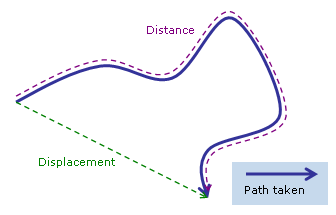
\includegraphics[scale=0.7]{Distancedisplacement}
            %     \fontfamily{cmss}\selectfont {
            %         \caption{Distance and displacement}
            %     }
            %     \label{fig:my_label}
            % \end{figure}
       
            
   		\item Cực trị tự do
            \begin{itemize}
                \item $f(x, y)$ đạt cực đại tương đối tại $M_{0}(x_{0}, y_{0})$ :  
                    \[f(x, y) = f(x_{0} + \Delta x, y_{0} + \Delta y) - f(x_{0}, y_{0}) \leqslant 0 \quad \forall (\Delta x, \Delta y) \to (0, 0)
                    \] 
                \item  $f(x, y)$ đạt cực tiểu tương đối tại $M_{0}(x_{0}, y_{0})$ :  
                \[f(x, y) = f(x_{0} + \Delta x, y_{0} + \Delta y) - f(x_{0}, y_{0}) \geqslant  0 \quad \forall (\Delta x, \Delta y) \to (0, 0)
                \] 
                \item $M_{0}$ là điểm tới hạn :
                    \[\dfrac{\partial f}{\partial x}(M_{0}) = \dfrac{\partial f}{\partial y}(M_{0}) = 0\]

                    hoặc một trong hai không tồn tại.
                \item Điều kiện cần :
                    Nếu hàm số có cực trị tại $M_{0}$ thì $M_{0}$ là điểm tới hạn.
                \item Điều kiện đủ :
                    Ta có điểm $M_{0}$ là điểm tới hạn của hàm số.

                    Để $M_{0}$ là điểm cực trị của hàm số:

                    Ta xét:
                        \[A = f''_{xx}(x_{0}, y_{0})\]
                        \[B = f''_{xy}(x_{0}, y_{0})\]
                        \[C = f''_{yy}(x_{0}, y_{0})\]
                    \indent Để $M_{0}$ là điểm cực trị của hàm số:
                        \[AC - B^{2} > 0\]
                    Nếu $A > 0$ hoặc $C > 0$ $\Rightarrow$ cực tiểu địa phương.

                    Nếu $A < 0$ hoặc $C < 0$ $\Rightarrow$ cực đại địa phương.
                    
                    Nếu $AC - B^{2} < 0$ $\Rightarrow$ không phải cực trị.

                    Nếu $AC - B^{2} = 0$ $\Rightarrow$ cũng có thể là có, cũng có thể là không.
            
            \end{itemize}
                
        \item Cực trị có điều kiện
            \begin{itemize}
                \item Nhân tử  Lagrange.
                    
                Xét tìm cực trị hàm số $f(x, y)$ với điều kiện $\varphi(x, y) = 0$
                \[L(x, y, \lambda) = f(x, y) + \lambda . \varphi(x, y)\]
                Ta có các điểm dừng:
                
            \end{itemize}
   		
            
    \end{enumerate}
    
\end{center}




}
\end{document}